% Отчёт по этапу 2 курсовой работы. Компилируется xelatex.
\documentclass[12pt,a4paper]{article}
\usepackage{fontspec}
\IfFontExistsTF{Times New Roman}{\setmainfont{Times New Roman}}{\setmainfont{Liberation Serif}}
\IfFontExistsTF{Courier New}{\setmonofont{Courier New}}{%
  \IfFontExistsTF{Liberation Mono}{\setmonofont{Liberation Mono}}{\setmonofont{DejaVu Sans Mono}}}
\IfFileExists{polyglossia.sty}{\usepackage{polyglossia}\setdefaultlanguage{russian}}{\usepackage[russian]{babel}}

\usepackage[left=25mm,right=15mm,top=20mm,bottom=20mm]{geometry}
\usepackage{longtable,array,booktabs,graphicx,float,caption,enumitem,xcolor}
\usepackage{listings}
\usepackage[unicode,hidelinks]{hyperref}
\setlist{nosep}
\setlength{\emergencystretch}{2em}
\setcounter{tocdepth}{2}
\captionsetup{labelsep=endash}
\captionsetup[table]{name=Таблица,justification=raggedright,singlelinecheck=false}
\captionsetup[figure]{name=Рисунок}
\newcolumntype{L}[1]{>{\raggedright\arraybackslash}p{#1}}
\graphicspath{{../img/}}

\lstdefinestyle{sql}{language=SQL, basicstyle=\ttfamily\scriptsize, columns=fullflexible,
  keepspaces=true, breaklines=true, breakatwhitespace=false, extendedchars=true,
  frame=single, framerule=0.3pt, rulecolor=\color{gray},
  keywordstyle=\bfseries, commentstyle=\color{gray}\itshape,
  morekeywords={RETURNS,LANGUAGE,PLPGSQL,TRIGGER,PROCEDURE,CALL,PERFORM,RAISE,EXCEPTION,
    NOTICE,LOOP,EXIT,IF,ELSIF,THEN,END,DECLARE,BEGIN,RETURN,QUERY,RETURNING,ENUM,TYPE,
    REFERENCES,RESTRICT,CASCADE,GENERATED,ALWAYS,STORED,INCLUDE,BOOLEAN,TEXT,SERIAL,
    BIGSERIAL,SMALLSERIAL,TIMESTAMPTZ,JSONB,COMMENT,EXECUTE,FUNCTION,FOUND,STABLE,IMMUTABLE}}
\lstset{style=sql}

\begin{document}

\begin{titlepage}
\centering
Университет ИТМО\\
Факультет программной инженерии и компьютерной техники

\vspace{60mm}
{\Large\bfseries Курсовая работа\par}
\vspace{4mm}
{\large Этап 2. Модель данных и её реализация в PostgreSQL\par}
\vspace{8mm}
{\large Информационная система «Бдительность»\par}

\vfill
\begin{flushright}
Выполнил: студент группы P3310\\
Мыц Иван Евгеньевич
\end{flushright}
\vspace{20mm}
Санкт-Петербург, 2026
\end{titlepage}

\tableofcontents
\newpage

\section{Задание}
\begin{enumerate}
  \item Сформировать ER-модель базы данных на основе описаний предметной области и
        прецедентов из предыдущего этапа. ER-модель должна включать не менее 10 сущностей
        и содержать хотя бы одно отношение вида «многие-ко-многим».
  \item Согласовать ER-модель с преподавателем. На основе ER-модели построить даталогическую модель.
  \item Реализовать даталогическую модель в реляционной СУБД PostgreSQL.
  \item Обеспечить целостность данных при помощи средств языка DDL и триггеров.
  \item Реализовать скрипты для создания, удаления базы данных, заполнения базы тестовыми данными.
  \item Предложить pl/pgsql-функции и процедуры для выполнения критически важных запросов,
        которые потребуются при последующей реализации прецедентов.
  \item Создать индексы на основе анализа использования базы данных в контексте описанных на
        первом этапе прецедентов. Обосновать полезность созданных индексов для реализации
        представленных на первом этапе бизнес-процессов.
  \item Составить отчёт.
\end{enumerate}

Исходными данными являются спецификация требований (SRS) версии 1.0 и модель прецедентов
UC01--UC23, разработанные на первом этапе. Ссылки на требования (U, C, S, SEC, REL и др.) и
прецеденты (UC) в настоящем отчёте соответствуют этой спецификации.

\section{ER-модель}\label{sec:er}

ER-модель построена по описанию предметной области (раздел 2.1 SRS), словарю терминов
(раздел 1.3 SRS) и спецификациям прецедентов (приложение А SRS). Модель представлена на
рисунке~\ref{fig:er} в нотации «вороньих лапок»: метка у конца связи обозначает кардинальность
со стороны соответствующей сущности (две черты --- ровно один, черта и кружок --- ноль или один,
«лапка» с кружком --- ноль или много, «лапка» с чертой --- один или много).

Модель содержит 16 сущностей. Связь «многие-ко-многим» между сущностями «Донос» и «Наказание»
выделена на рисунке красным цветом. Статус благонадёжности жильца не является атрибутом:
он однозначно определяется значением ИЛ и вычисляется при запросе. Диаграмма в исходном размере приложена
к отчёту в файле \texttt{img/er.pdf}.

\begin{figure}[tbp]
  \centering
  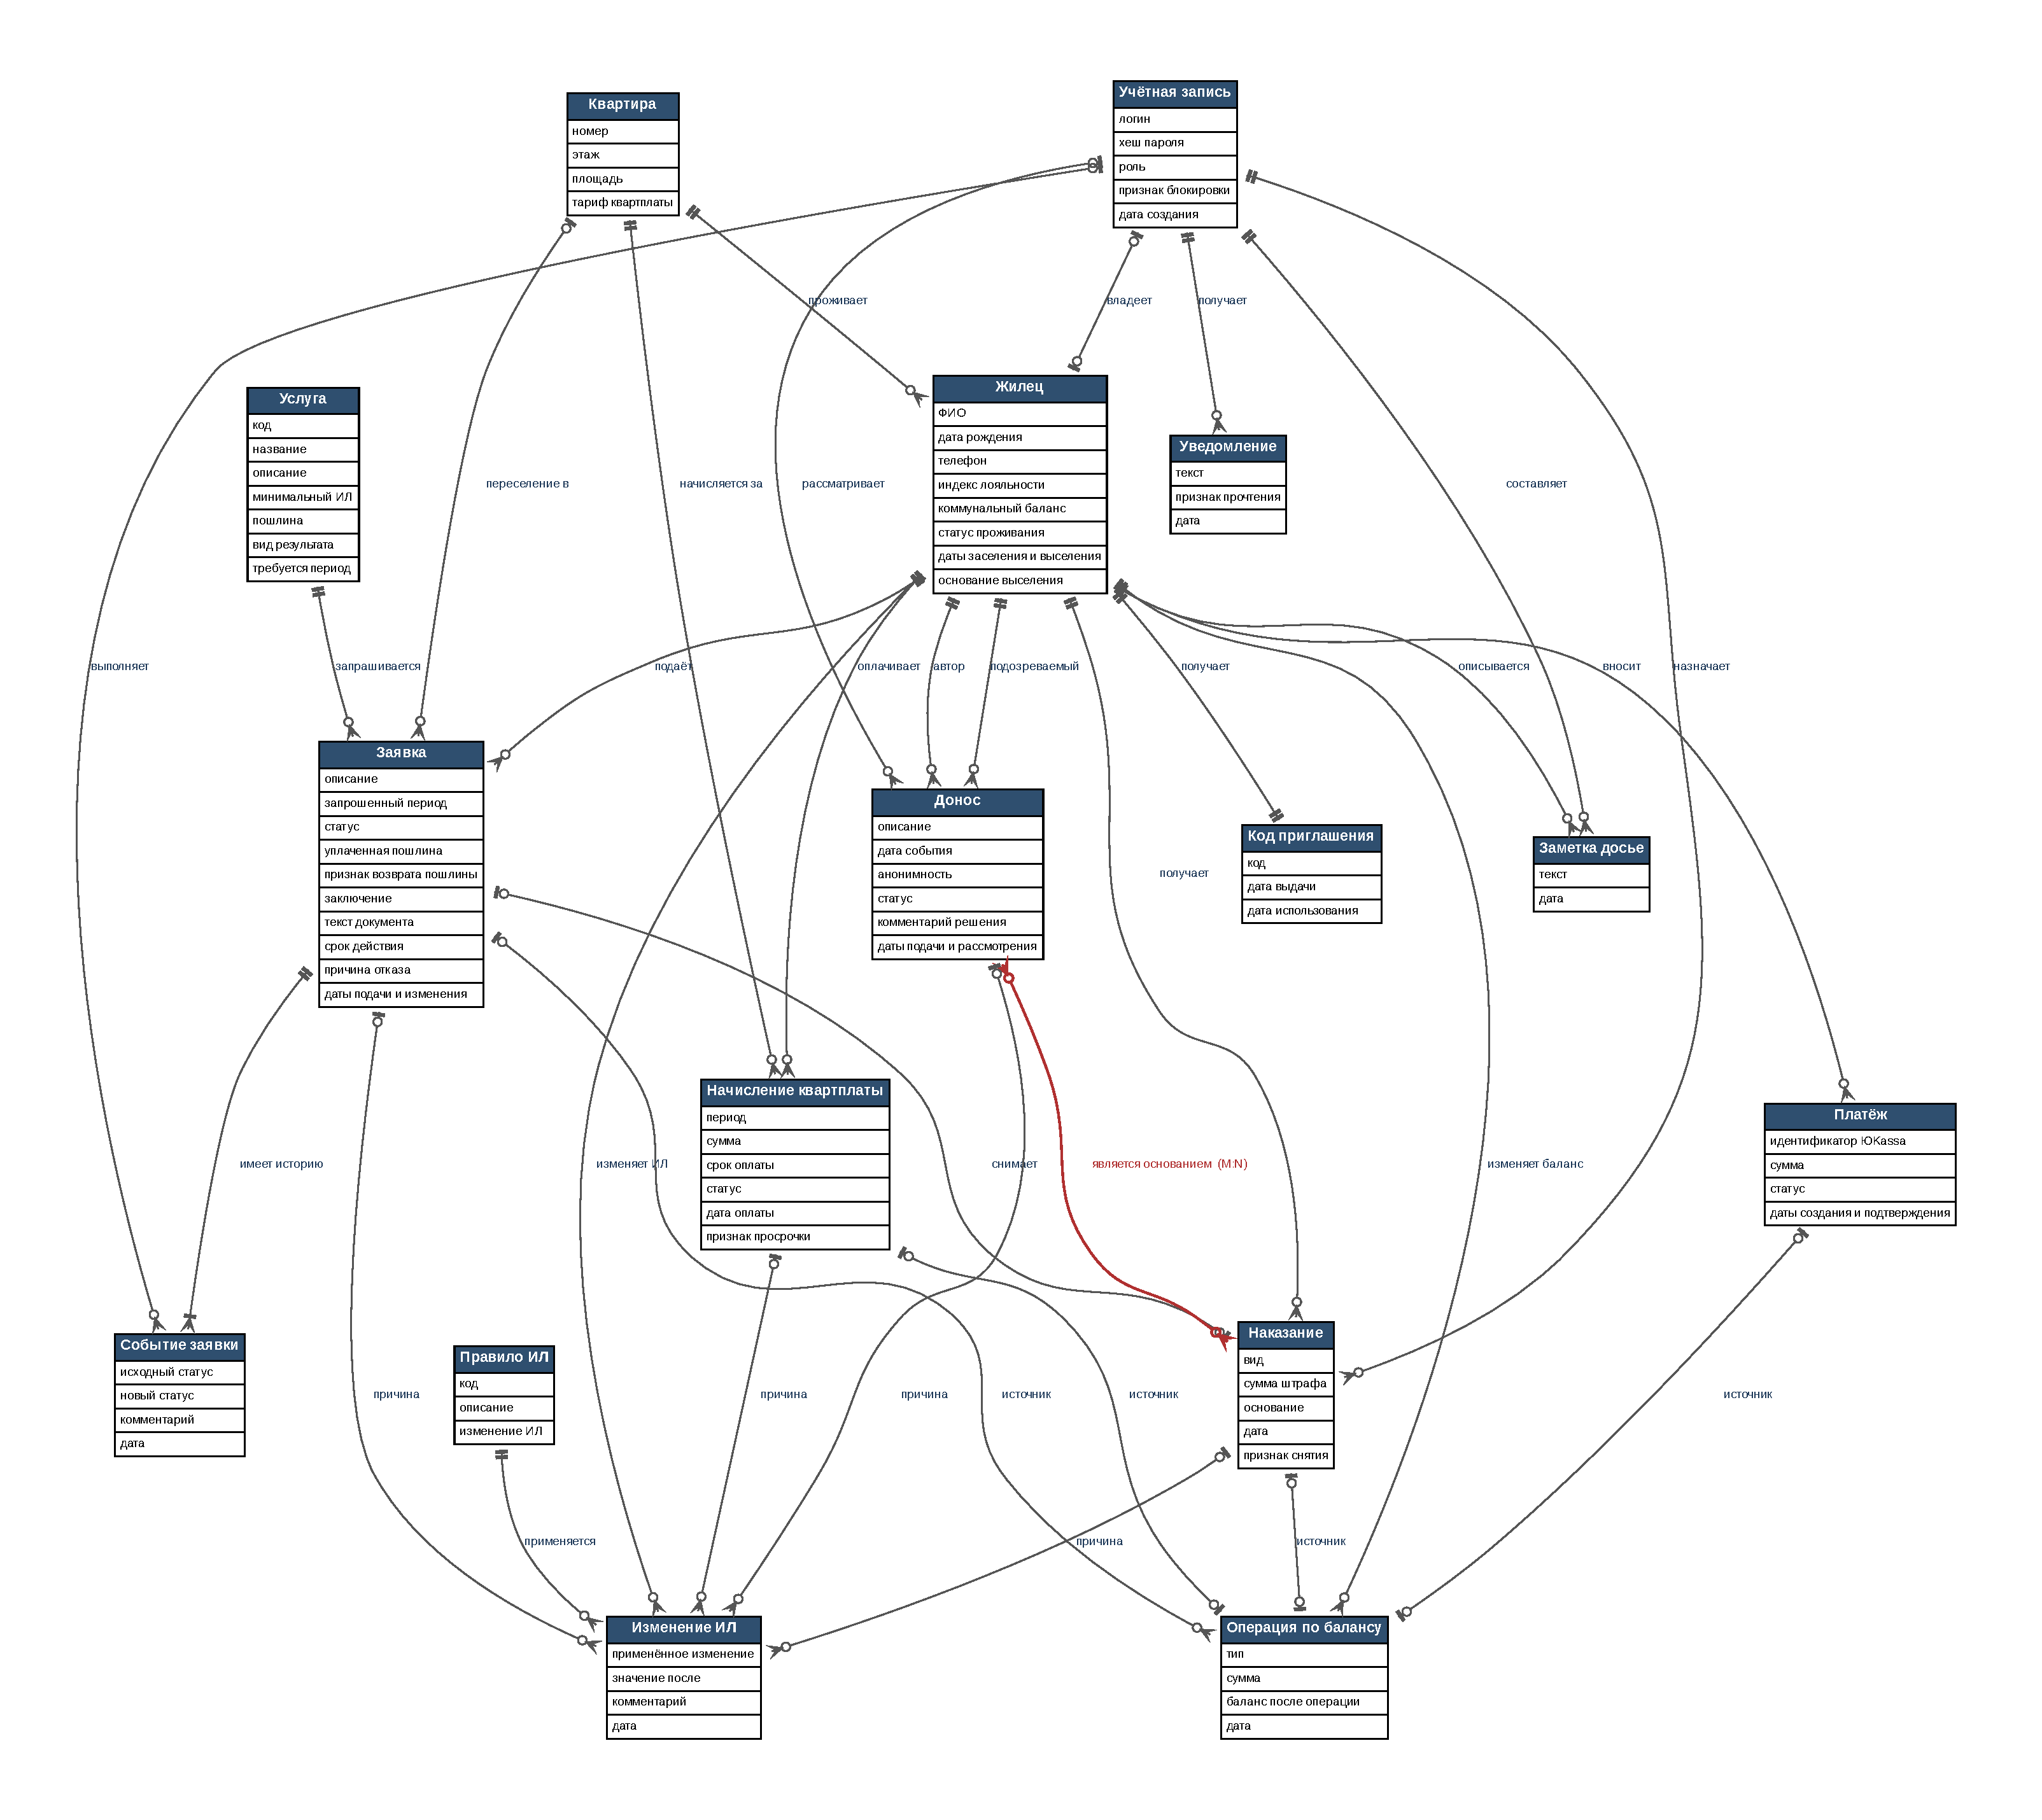
\includegraphics[width=\textwidth]{er.pdf}
  \caption{ER-модель базы данных}
  \label{fig:er}
\end{figure}

\begin{longtable}{L{37.2mm} L{66.6mm} L{52.9mm}}
\caption{Сущности ER-модели}\label{tab:entities}\\
\toprule \textbf{Сущность} & \textbf{Назначение} & \textbf{Основные атрибуты} \\ \midrule
\endfirsthead
\toprule \textbf{Сущность} & \textbf{Назначение} & \textbf{Основные атрибуты} \\ \midrule
\endhead
\bottomrule
\endfoot
Учётная запись & Данные для входа пользователя: жильца или управляющего. & логин, хеш пароля, роль, признак блокировки \\
Квартира & Жилое помещение дома, за которое начисляется квартплата. & номер, этаж, площадь, тариф \\
Жилец & Гражданин, проживающий в доме; хранит анкету, ИЛ и коммунальный баланс. & ФИО, дата рождения, телефон, ИЛ, баланс, статус \\
Код приглашения & Одноразовый код для активации учётной записи жильца. & код, даты выдачи и использования \\
Услуга & Услуга из фиксированного перечня (SV01--SV09). & код, название, минимальный ИЛ, пошлина, вид результата \\
Заявка & Обращение жильца за услугой и его результат. & статус, пошлина, заключение, документ, срок действия \\
Событие заявки & Запись истории обработки заявки: смена статуса, вопрос или ответ. & исходный и новый статус, комментарий, дата \\
Донос & Сообщение жильца о нарушении, допущенном другим жильцом. & описание, анонимность, статус, решение \\
Наказание & Мера, назначенная жильцу: предупреждение, штраф, выселение. & вид, сумма, основание, признак снятия \\
Платёж & Пополнение баланса через ЮKassa. & идентификатор ЮKassa, сумма, статус \\
Начисление квартплаты & Ежемесячное начисление за квартиру. & период, сумма, срок оплаты, статус \\
Операция по балансу & Запись журнала изменений коммунального баланса. & тип, сумма, баланс после операции \\
Правило ИЛ & Правило изменения индекса лояльности (RL01--RL07). & код, описание, величина изменения \\
Изменение ИЛ & Запись журнала изменений индекса лояльности. & применённое изменение, значение после \\
Заметка досье & Наблюдение управляющего о жильце. & текст, дата \\
Уведомление & Сообщение пользователю о событии в системе. & текст, признак прочтения \\
\end{longtable}
\begin{longtable}{L{45.1mm} L{32.3mm} L{79.4mm}}
\caption{Связи ER-модели}\label{tab:relations}\\
\toprule \textbf{Связь} & \textbf{Кардинальность} & \textbf{Смысл} \\ \midrule
\endfirsthead
\toprule \textbf{Связь} & \textbf{Кардинальность} & \textbf{Смысл} \\ \midrule
\endhead
\bottomrule
\endfoot
Учётная запись — Жилец & 0..1 : 0..1 & Жилец получает учётную запись после активации; у управляющего записи жильца нет. \\
Квартира — Жилец & 1 : 0..* & Жилец проживает в квартире; в квартире одновременно проживает не более одного жильца, выселенные жильцы сохраняют связь с последней квартирой. \\
Жилец — Код приглашения & 1 : 1 & При заселении жильцу выдаётся код приглашения. \\
Жилец — Заявка & 1 : 0..* & Жилец подаёт заявки. \\
Услуга — Заявка & 1 : 0..* & Заявка подаётся на одну услугу. \\
Квартира — Заявка & 0..1 : 0..* & Заявка на переселение (SV07) указывает целевую квартиру. \\
Заявка — Событие заявки & 1 : 1..* & Заявка имеет историю обработки. \\
Учётная запись — Событие заявки & 0..1 : 0..* & Пользователь, изменивший статус заявки. \\
Жилец — Донос & 1 : 0..* & Жилец является автором доноса. \\
Жилец — Донос & 1 : 0..* & Жилец является подозреваемым по доносу. \\
Учётная запись — Донос & 0..1 : 0..* & Управляющий рассматривает донос. \\
Жилец — Наказание & 1 : 0..* & Жилец получает наказание. \\
Учётная запись — Наказание & 1 : 0..* & Управляющий назначает наказание. \\
\textbf{Донос — Наказание} & \textbf{0..* : 0..*} & \textbf{Наказание назначается по одному или нескольким подтверждённым доносам об одном нарушении; по одному доносу может быть назначено несколько наказаний (например, штраф и предупреждение).} \\
Заявка — Наказание & 0..1 : 0..1 & Выполненная заявка SV09 снимает предупреждение. \\
Жилец — Платёж & 1 : 0..* & Жилец пополняет баланс. \\
Жилец — Начисление квартплаты & 1 : 0..* & Квартплата начисляется жильцу. \\
Квартира — Начисление квартплаты & 1 : 0..* & Квартплата начисляется за квартиру. \\
Жилец — Операция по балансу & 1 : 0..* & Операция изменяет баланс жильца. \\
Платёж, Начисление, Заявка, Наказание — Операция по балансу & 0..1 : 0..1 (для заявки 0..1 : 0..*) & Источник операции: пополнение, оплата квартплаты, пошлина или её возврат, штраф. \\
Жилец — Изменение ИЛ & 1 : 0..* & Изменение относится к жильцу. \\
Правило ИЛ — Изменение ИЛ & 1 : 0..* & Изменение выполняется по правилу. \\
Донос, Наказание, Начисление, Заявка — Изменение ИЛ & 0..1 : 0..* & Причина изменения ИЛ. \\
Жилец — Заметка досье & 1 : 0..* & Заметка описывает жильца. \\
Учётная запись — Заметка досье & 1 : 0..* & Управляющий составляет заметку. \\
Учётная запись — Уведомление & 1 : 0..* & Пользователь получает уведомления. \\
\end{longtable}
Сущности «Операция по балансу» и «Изменение ИЛ» выделены как журналы: текущие значения
баланса и ИЛ жильца всегда равны сумме записей журнала, а сами записи не изменяются (требование
S013 SRS). Это позволяет восстановить историю изменений (UC05, UC12) и проверить корректность
текущих значений.

\section{Даталогическая модель}\label{sec:datalogical}

Даталогическая модель (рисунок~\ref{fig:datalogical}) получена из ER-модели по следующим правилам.
\begin{enumerate}
  \item Каждая сущность преобразована в таблицу с суррогатным первичным ключом \texttt{id}.
        Для справочника правил ИЛ используется естественный ключ \texttt{code}.
  \item Связи «один-ко-многим» реализованы внешними ключами на стороне «многие».
  \item Связи «один-к-одному» реализованы внешним ключом с ограничением \texttt{UNIQUE}
        (столбец \texttt{account\_\allowbreak{}id} таблицы \texttt{resident}, столбец \texttt{resident\_\allowbreak{}id}
        таблицы \texttt{invitation}, столбец \texttt{payment\_\allowbreak{}id} таблицы \texttt{balance\_\allowbreak{}operation} и др.).
  \item Связь «многие-ко-многим» «Донос — Наказание» реализована ассоциативной таблицей
        \texttt{punishment\_\allowbreak{}basis} с составным первичным ключом.
  \item Атрибуты с фиксированным набором значений (роль, статусы, виды наказаний, типы операций)
        реализованы перечислимыми типами PostgreSQL (\texttt{CREATE TYPE \dots{} AS ENUM}).
  \item Статус благонадёжности не хранится, а вычисляется по ИЛ функцией
        \texttt{reliability\_\allowbreak{}status} (пороги из таблицы статусов SRS, требование S011).
  \item Задолженность хранится как отрицательное значение \texttt{resident.\allowbreak{}balance}: при пополнении
        баланса задолженность погашается автоматически (требование S004 SRS).
\end{enumerate}

Модель находится в третьей нормальной форме, за одним осознанным исключением.
Столбцы \texttt{resident.\allowbreak{}balance} и \texttt{resident.\allowbreak{}loyalty\_\allowbreak{}index} дублируют суммы журналов
\texttt{balance\_\allowbreak{}operation} и \texttt{loyalty\_\allowbreak{}change}. Они хранятся для быстрой проверки условий
подачи заявок и сортировки очереди; их согласованность с журналами обеспечивается триггерами
(раздел~\ref{sec:integrity}).

Не являются избыточными столбцы \texttt{rent\_\allowbreak{}charge.\allowbreak{}apartment\_\allowbreak{}id} и
\texttt{service\_\allowbreak{}request.\allowbreak{}fee\_\allowbreak{}paid}: первый фиксирует квартиру на момент начисления, которая может
измениться после переселения, второй --- пошлину, уплаченную в момент подачи заявки.
Диаграмма в исходном размере приложена в файле \texttt{img/datalogical.pdf}.

\begin{figure}[tbp]
  \centering
  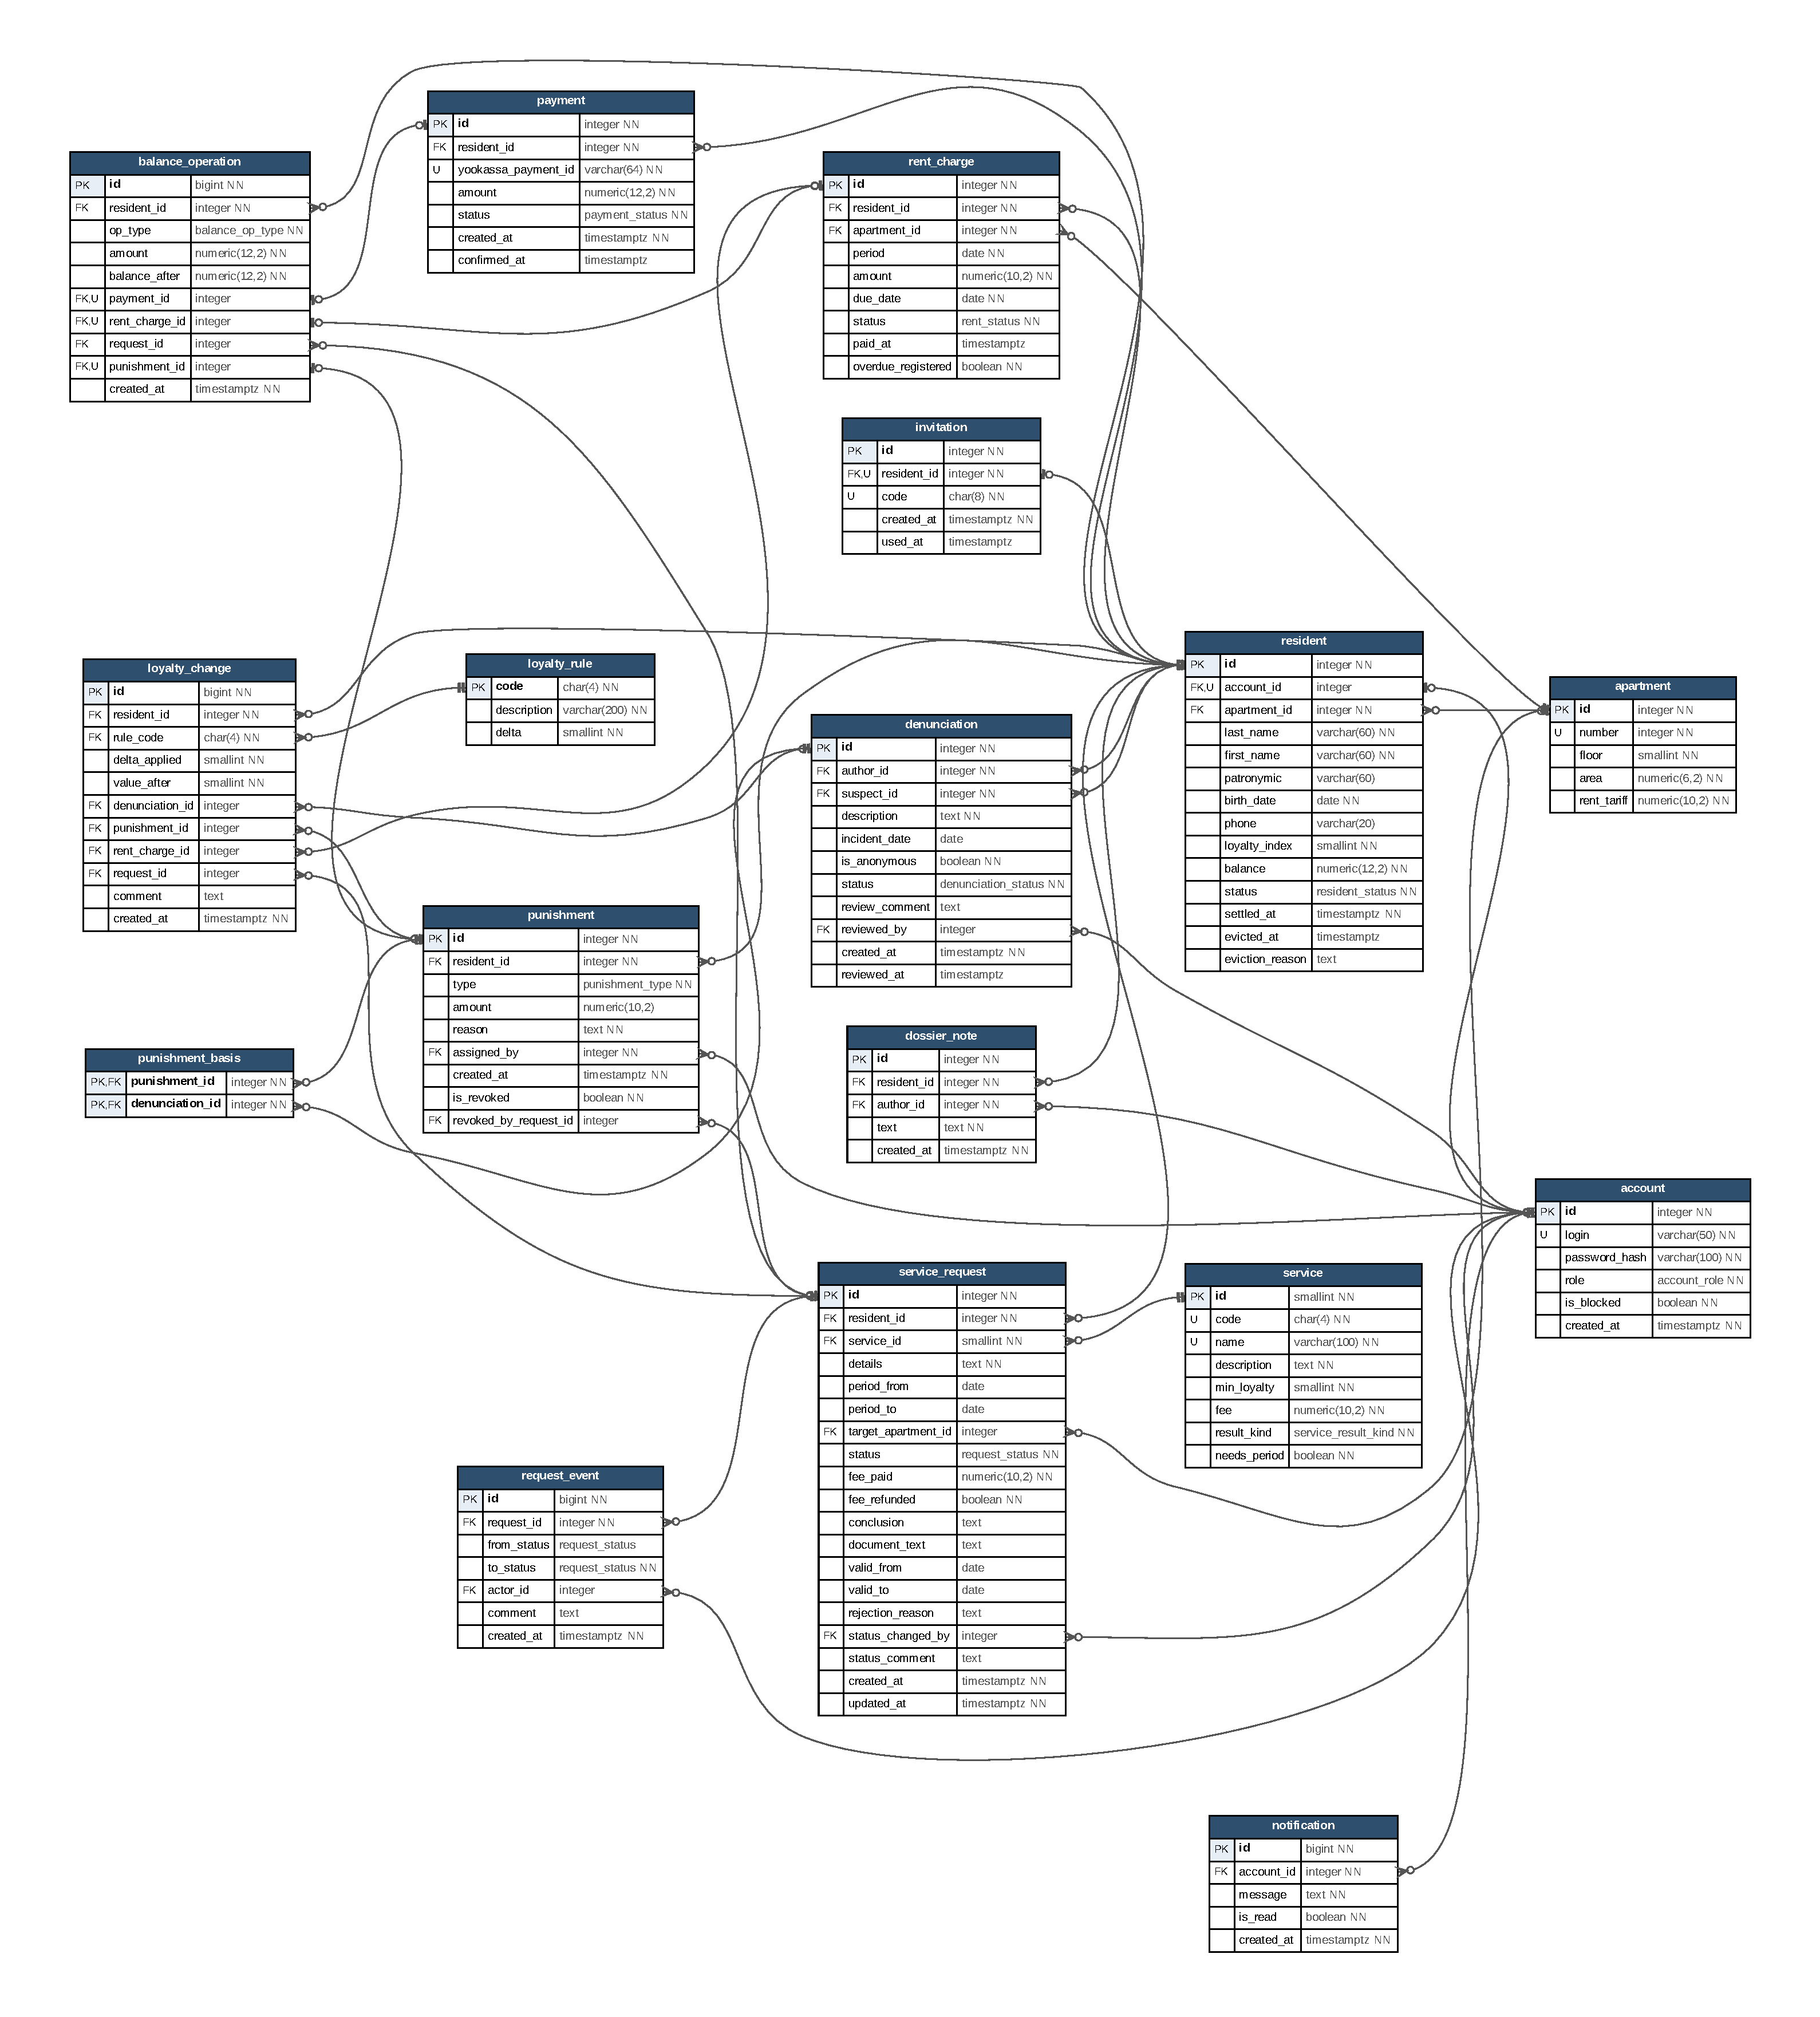
\includegraphics[width=\textwidth]{datalogical.pdf}
  \caption{Даталогическая модель базы данных (PK --- первичный ключ, FK --- внешний ключ,
           U --- уникальное значение, NN --- NOT NULL)}
  \label{fig:datalogical}
\end{figure}

\begin{longtable}{L{30.5mm} L{33.3mm} L{34.3mm} L{54.3mm}}
\caption{Таблицы базы данных}\label{tab:tables}\\
\toprule \textbf{Таблица} & \textbf{Сущность} & \textbf{Первичный ключ} & \textbf{Внешние ключи} \\ \midrule
\endfirsthead
\toprule \textbf{Таблица} & \textbf{Сущность} & \textbf{Первичный ключ} & \textbf{Внешние ключи} \\ \midrule
\endhead
\bottomrule
\endfoot
\texttt{account} & Учётная запись & \texttt{id} & — \\
\texttt{apartment} & Квартира & \texttt{id} & — \\
\texttt{resident} & Жилец & \texttt{id} & \texttt{account\_\allowbreak{}id (U), apartment\_\allowbreak{}id} \\
\texttt{invitation} & Код приглашения & \texttt{id} & \texttt{resident\_\allowbreak{}id (U)} \\
\texttt{service} & Услуга & \texttt{id} & — \\
\texttt{service\_\allowbreak{}request} & Заявка & \texttt{id} & \texttt{resident\_\allowbreak{}id, service\_\allowbreak{}id, target\_\allowbreak{}apartment\_\allowbreak{}id, status\_\allowbreak{}changed\_\allowbreak{}by} \\
\texttt{request\_\allowbreak{}event} & Событие заявки & \texttt{id} & \texttt{request\_\allowbreak{}id, actor\_\allowbreak{}id} \\
\texttt{denunciation} & Донос & \texttt{id} & \texttt{author\_\allowbreak{}id, suspect\_\allowbreak{}id, reviewed\_\allowbreak{}by} \\
\texttt{punishment} & Наказание & \texttt{id} & \texttt{resident\_\allowbreak{}id, assigned\_\allowbreak{}by, revoked\_\allowbreak{}by\_\allowbreak{}request\_\allowbreak{}id} \\
\texttt{punishment\_\allowbreak{}basis} & Связь M:N «Донос — Наказание» & \texttt{(punishment\_\allowbreak{}id, denunciation\_\allowbreak{}id)} & \texttt{punishment\_\allowbreak{}id, denunciation\_\allowbreak{}id} \\
\texttt{payment} & Платёж & \texttt{id} & \texttt{resident\_\allowbreak{}id} \\
\texttt{rent\_\allowbreak{}charge} & Начисление квартплаты & \texttt{id} & \texttt{resident\_\allowbreak{}id, apartment\_\allowbreak{}id} \\
\texttt{balance\_\allowbreak{}operation} & Операция по балансу & \texttt{id} & \texttt{resident\_\allowbreak{}id, payment\_\allowbreak{}id (U), rent\_\allowbreak{}charge\_\allowbreak{}id (U), request\_\allowbreak{}id, punishment\_\allowbreak{}id (U)} \\
\texttt{loyalty\_\allowbreak{}rule} & Правило ИЛ & \texttt{code} & — \\
\texttt{loyalty\_\allowbreak{}change} & Изменение ИЛ & \texttt{id} & \texttt{resident\_\allowbreak{}id, rule\_\allowbreak{}code, denunciation\_\allowbreak{}id, punishment\_\allowbreak{}id, rent\_\allowbreak{}charge\_\allowbreak{}id, request\_\allowbreak{}id} \\
\texttt{dossier\_\allowbreak{}note} & Заметка досье & \texttt{id} & \texttt{resident\_\allowbreak{}id, author\_\allowbreak{}id} \\
\texttt{notification} & Уведомление & \texttt{id} & \texttt{account\_\allowbreak{}id} \\
\end{longtable}
\section{Реализация в PostgreSQL}\label{sec:impl}

Даталогическая модель реализована в виде набора SQL-скриптов (таблица~\ref{tab:scripts}).
Скрипты не создают отдельную базу данных и схему: объекты создаются в текущей схеме
(\texttt{search\_\allowbreak{}path}). Это позволяет выполнять скрипты на сервере helios, где студенту
доступна личная схема в базе \texttt{studs}, а команда \texttt{CREATE DATABASE} недоступна.
Скрипт удаления удаляет все созданные объекты. Скрипты проверены на PostgreSQL 16 и используют
возможности, доступные начиная с PostgreSQL 11 (процедуры, \texttt{INCLUDE} в индексах).

\begin{longtable}{L{38.3mm} L{122.9mm}}
\caption{Скрипты базы данных}\label{tab:scripts}\\
\toprule \textbf{Файл} & \textbf{Назначение} \\ \midrule
\endfirsthead
\toprule \textbf{Файл} & \textbf{Назначение} \\ \midrule
\endhead
\bottomrule
\endfoot
\texttt{install.\allowbreak{}sql} & Создание базы целиком: последовательно выполняет скрипты 01--04. \\
\texttt{00\_\allowbreak{}drop.sql} & Удаление всех объектов: представлений, таблиц, функций, процедур и типов. Повторный запуск безопасен. \\
\texttt{01\_\allowbreak{}create.sql} & Перечислимые типы, таблицы, ограничения целостности, комментарии и справочные данные (услуги, правила ИЛ). \\
\texttt{02\_\allowbreak{}triggers.sql} & Триггерные и вспомогательные функции, триггеры. \\
\texttt{03\_\allowbreak{}functions.sql} & Функции и процедуры прецедентов, представления. \\
\texttt{04\_\allowbreak{}indexes.sql} & Индексы. \\
\texttt{05\_\allowbreak{}fill.sql} & Тестовые данные: 30 квартир, 24 жильца, управляющий, платежи, квартплата за два месяца, 13 заявок во всех статусах, 23 доноса, 15 наказаний. \\
\texttt{06\_\allowbreak{}fill\_\allowbreak{}bulk.sql} & Необязательные массовые данные для проверки индексов: 100 квартир, 300 жильцов, 10\,000 заявок, 10\,000 доносов (требование PRF002 SRS). \\
\texttt{07\_\allowbreak{}tests.sql} & Проверка ограничений целостности; все изменения откатываются. \\
\end{longtable}
Порядок развёртывания на сервере helios:
\begin{lstlisting}[language=bash]
cd sql
psql -h pg -d studs -f 00_drop.sql      # удалить предыдущую версию (при необходимости)
psql -h pg -d studs -f install.sql      # создать таблицы, триггеры, функции, индексы
psql -h pg -d studs -f 05_fill.sql      # заполнить тестовыми данными
psql -h pg -d studs -f 07_tests.sql     # проверить ограничения целостности
\end{lstlisting}

Тестовые данные создаются через функции прецедентов (раздел~\ref{sec:functions}), поэтому
журналы операций, история заявок, история ИЛ и уведомления согласованы между собой.
Для входа в систему используются учётные записи \texttt{manager / manager123} (управляющий)
и \texttt{gromov}, \texttt{belova} и др. \texttt{/ resident123} (жильцы); в базе хранятся
bcrypt-хеши паролей.

\section{Обеспечение целостности данных}\label{sec:integrity}

\subsection{Средства DDL}

\begin{longtable}{L{48.4mm} L{112.8mm}}
\caption{Ограничения целостности, заданные средствами DDL}\label{tab:ddl}\\
\toprule \textbf{Средство} & \textbf{Применение} \\ \midrule
\endfirsthead
\toprule \textbf{Средство} & \textbf{Применение} \\ \midrule
\endhead
\bottomrule
\endfoot
Перечислимые типы & Допустимые значения ролей, статусов заявок, доносов, платежей, начислений, видов наказаний и типов операций. \\
\texttt{NOT NULL} & Обязательные атрибуты всех сущностей. \\
\texttt{PRIMARY KEY}, \texttt{FOREIGN KEY} & Ссылочная целостность. Для связей, удаление по которым недопустимо (жилец, заявка, донос), задано \texttt{ON DELETE RESTRICT}; для зависимых данных (код приглашения, заметки, уведомления) --- \texttt{ON DELETE CASCADE}. \\
\texttt{UNIQUE} & Логин, код приглашения, номер квартиры, идентификатор платежа ЮKassa, одно начисление на квартиру и на жильца за период (переселившийся жилец не платит дважды), одна операция на платёж, начисление и штраф (REL002). \\
Частичные уникальные индексы & \texttt{uq\_\allowbreak{}account\_\allowbreak{}single\_\allowbreak{}manager} --- в системе один управляющий; \texttt{uq\_\allowbreak{}resident\_\allowbreak{}active\_\allowbreak{}apartment} --- в квартире проживает не более одного жильца. \\
\texttt{CHECK} на значения & ИЛ в диапазоне 0--100 (S010), положительные суммы платежей, неотрицательные пошлины и тарифы, формат логина, кода приглашения, кодов услуг и правил, начало периода начисления --- первое число месяца. \\
\texttt{CHECK} на сочетания & Донос не может быть подан на себя (U026); статус «Выселен» тогда и только тогда, когда указана дата выселения; выполненная заявка имеет заключение, отклонённая --- причину; сумма указывается только у штрафа; снять можно только предупреждение; знак суммы операции и ссылка на источник соответствуют типу операции. \\
\end{longtable}
\subsection{Триггеры}
Правила, которые нельзя выразить декларативно, реализованы триггерами (таблица~\ref{tab:triggers}).
Триггеры обеспечивают выполнение бизнес-правил независимо от того, через какую функцию или
напрямую изменяются данные.

Ключевое решение --- \emph{применение журналов}. Баланс и ИЛ жильца изменяются только вставкой
записи в \texttt{balance\_\allowbreak{}operation} или \texttt{loyalty\_\allowbreak{}change}; триггер вставки вычисляет новое
значение и обновляет строку жильца. Прямое изменение \texttt{resident.\allowbreak{}balance} или
\texttt{resident.\allowbreak{}loyalty\_\allowbreak{}index} отклоняется триггером \texttt{resident\_\allowbreak{}guard}, который различает
вызов из триггера журнала по глубине вложенности триггеров (\texttt{pg\_\allowbreak{}trigger\_\allowbreak{}depth()}).
Таким образом текущие значения всегда совпадают с суммой записей журналов.

\begin{longtable}{L{33.3mm} L{30.5mm} L{20.4mm} L{48.1mm} L{15.7mm}}
\caption{Триггеры}\label{tab:triggers}\\
\toprule \textbf{Триггер} & \textbf{Таблица} & \textbf{Событие} & \textbf{Назначение} & \textbf{SRS} \\ \midrule
\endfirsthead
\toprule \textbf{Триггер} & \textbf{Таблица} & \textbf{Событие} & \textbf{Назначение} & \textbf{SRS} \\ \midrule
\endhead
\bottomrule
\endfoot
\texttt{balance\_\allowbreak{}operation\_\allowbreak{}apply} & \texttt{balance\_\allowbreak{}operation} & BEFORE INSERT & Применяет операцию к балансу жильца, запрещает уход в минус, кроме штрафов & S005, U017 \\
\texttt{loyalty\_\allowbreak{}change\_\allowbreak{}apply} & \texttt{loyalty\_\allowbreak{}change} & BEFORE INSERT & Изменяет ИЛ по правилу, ограничивает его диапазоном 0--100 & S009, S010 \\
\texttt{*\_\allowbreak{}immutable} & \texttt{balance\_\allowbreak{}operation, loyalty\_\allowbreak{}change, request\_\allowbreak{}event} & BEFORE UPDATE, DELETE & Запрещает изменение и удаление записей журналов & S013 \\
\texttt{resident\_\allowbreak{}guard} & \texttt{resident} & BEFORE INSERT, UPDATE & Задаёт начальные значения, запрещает дату рождения в будущем, изменение баланса и ИЛ в обход журналов и восстановление выселенного жильца & S008 \\
\texttt{resident\_\allowbreak{}after\_\allowbreak{}update} & \texttt{resident} & AFTER UPDATE & Уведомляет об изменении ИЛ и о падении ИЛ ниже 10; блокирует учётную запись при выселении & S012, U030, C021 \\
\texttt{account\_\allowbreak{}guard} & \texttt{account} & BEFORE UPDATE & Запрещает смену роли & SEC002 \\
\texttt{invitation\_\allowbreak{}guard} & \texttt{invitation} & BEFORE UPDATE & Запрещает повторное использование кода & U002 \\
\texttt{request\_\allowbreak{}before\_\allowbreak{}insert} & \texttt{service\_\allowbreak{}request} & BEFORE INSERT & Проверяет статус жильца, ИЛ, задолженность, наличие периода, предупреждения (SV09) и свободной квартиры для переселения (SV07); фиксирует пошлину & U015, U017 \\
\texttt{request\_\allowbreak{}after\_\allowbreak{}insert} & \texttt{service\_\allowbreak{}request} & AFTER INSERT & Списывает пошлину, создаёт первую запись истории & U016, S006 \\
\texttt{request\_\allowbreak{}before\_\allowbreak{}update} & \texttt{service\_\allowbreak{}request} & BEFORE UPDATE & Проверяет переход по модели состояний заявки, запрещает менять заявителя, услугу, пошлину и результат & S006 \\
\texttt{request\_\allowbreak{}after\_\allowbreak{}update} & \texttt{service\_\allowbreak{}request} & AFTER UPDATE & Записывает историю, возвращает пошлину, уведомляет жильца & S006, U018, U030 \\
\texttt{denunciation\_\allowbreak{}before} & \texttt{denunciation} & BEFORE INSERT, UPDATE & Проверяет, что участники проживают в доме и дата нарушения не в будущем; запрещает повторное рассмотрение и изменение содержания; проверяет роль рассматривающего & S007 \\
\texttt{denunciation\_\allowbreak{}after\_\allowbreak{}update} & \texttt{denunciation} & AFTER UPDATE & Изменяет ИЛ неанонимного доносчика (RL01, RL02), уведомляет его & S009, U028 \\
\texttt{punishment\_\allowbreak{}before} & \texttt{punishment} & BEFORE INSERT, UPDATE & Проверяет роль управляющего и статус жильца, запрещает изменение назначенного наказания & C013 \\
\texttt{punishment\_\allowbreak{}after\_\allowbreak{}insert} & \texttt{punishment} & AFTER INSERT & Применяет последствия: ИЛ (RL05, RL06), списание штрафа, выселение & S005, C021 \\
\texttt{punishment\_\allowbreak{}basis\_\allowbreak{}check} & \texttt{punishment\_\allowbreak{}basis} & BEFORE INSERT, UPDATE & Основанием может быть только подтверждённый донос на наказываемого жильца & C013 \\
\texttt{payment\_\allowbreak{}before\_\allowbreak{}update} & \texttt{payment} & BEFORE UPDATE & Меняет статус только из PENDING, фиксирует время подтверждения & S003 \\
\texttt{payment\_\allowbreak{}after\_\allowbreak{}update} & \texttt{payment} & AFTER UPDATE & Зачисляет средства ровно один раз & S003, REL002 \\
\texttt{rent\_\allowbreak{}before\_\allowbreak{}update} & \texttt{rent\_\allowbreak{}charge} & BEFORE UPDATE & Запрещает отмену оплаты и изменение параметров начисления & S001 \\
\texttt{rent\_\allowbreak{}after\_\allowbreak{}update} & \texttt{rent\_\allowbreak{}charge} & AFTER UPDATE & Применяет RL03 при оплате в срок и RL04 при регистрации просрочки & S002 \\
\texttt{dossier\_\allowbreak{}note\_\allowbreak{}check} & \texttt{dossier\_\allowbreak{}note} & BEFORE INSERT, UPDATE & Заметки добавляет только управляющий & C023 \\
\end{longtable}
\subsection{Проверка}
Скрипт \texttt{07\_\allowbreak{}tests.sql} выполняет 33 попытки нарушить ограничения целостности и 3 проверки
согласованности данных. Все 36 проверок пройдены: каждая попытка нарушения отклонена с
сообщением об ошибке, а баланс и ИЛ всех жильцов совпадают с журналами.
\begin{enumerate}[label=\arabic*., itemsep=0pt]
\small
  \item Донос на самого себя.
  \item Прямое изменение баланса.
  \item Прямое изменение ИЛ.
  \item Создание жильца с ИЛ, отличным от 50.
  \item Второй управляющий.
  \item Заселение в занятую квартиру.
  \item Повторная активация по коду.
  \item Заявка при недостаточном ИЛ.
  \item Заявка при задолженности.
  \item Заявка выселенного жильца.
  \item Разрешение без указания периода.
  \item Недопустимый переход статуса заявки.
  \item Отмена заявки, принятой в работу.
  \item Изменение пошлины в заявке.
  \item Действие управляющего от имени жильца.
  \item Повторное рассмотрение доноса.
  \item Изменение текста доноса.
  \item Наказание по нерассмотренному доносу.
  \item Наказание по доносу на другого жильца.
  \item Штраф без суммы.
  \item Оплата квартплаты при недостатке средств.
  \item Изменение журнала операций по балансу.
  \item Удаление записи истории ИЛ.
  \item Удаление истории заявки.
  \item Повторное изменение статуса платежа.
  \item Отмена оплаты квартплаты.
  \item Восстановление выселенного жильца.
  \item Снятие предупреждения при их отсутствии.
  \item Заметка в досье от жильца.
  \item Отрицательная сумма платежа.
  \item Переселение в занятую квартиру.
  \item Дата нарушения в будущем.
  \item Дата рождения в будущем.
  \item Повторная обработка платежа не меняет баланс.
  \item Баланс всех жильцов совпадает с журналом операций.
  \item ИЛ всех жильцов совпадает с журналом изменений.
\end{enumerate}

\section{Функции и процедуры}\label{sec:functions}

Для каждого прецедента, изменяющего данные или требующего сложной выборки, реализована
функция или процедура PL/pgSQL (таблица~\ref{tab:functions}). Функции выполняют операцию прецедента
одним вызовом и одной транзакцией (REL001 SRS), а проверку правил и побочные эффекты (списание
средств, изменение ИЛ, запись истории, уведомления) берут на себя триггеры. Это исключает
дублирование правил между функциями и серверной частью приложения.

\begin{longtable}{L{40.0mm} L{19.1mm} L{21.0mm} L{72.4mm}}
\caption{Функции и процедуры прецедентов}\label{tab:functions}\\
\toprule \textbf{Имя} & \textbf{Вид} & \textbf{Прецедент} & \textbf{Назначение} \\ \midrule
\endfirsthead
\toprule \textbf{Имя} & \textbf{Вид} & \textbf{Прецедент} & \textbf{Назначение} \\ \midrule
\endhead
\bottomrule
\endfoot
\texttt{settle\_\allowbreak{}resident} & функция & UC13 & Заселяет жильца в свободную квартиру, создаёт код приглашения. \\
\texttt{activate\_\allowbreak{}account} & функция & UC01 & Проверяет код, создаёт учётную запись жильца, отмечает код использованным. \\
\texttt{evict\_\allowbreak{}resident} & процедура & UC14 & Выселяет жильца: назначает наказание «выселение», последствия выполняют триггеры. \\
\texttt{register\_\allowbreak{}payment} & функция & UC04 & Регистрирует платёж, созданный в ЮKassa. \\
\texttt{apply\_\allowbreak{}payment\_\allowbreak{}status} & функция & UC04 & Применяет статус платежа из API ЮKassa; идемпотентна (REL002, COM003). \\
\texttt{accrue\_\allowbreak{}rent} & процедура & S001 & Начисляет квартплату за месяц жильцам, заселённым до конца месяца, без повторных начислений. \\
\texttt{register\_\allowbreak{}overdue\_\allowbreak{}rent} & функция & S002 & Регистрирует просрочку неоплаченных начислений жильцов с активированной учётной записью; возвращает их число. \\
\texttt{pay\_\allowbreak{}rent} & процедура & UC06 & Оплачивает начисление квартплаты с баланса. \\
\texttt{available\_\allowbreak{}services} & функция & UC03 & Перечень услуг с признаком доступности по ИЛ жильца. \\
\texttt{submit\_\allowbreak{}request} & функция & UC07 & Подаёт заявку на услугу по коду услуги. \\
\texttt{cancel\_\allowbreak{}request} & процедура & UC08 & Отменяет заявку в статусе «Подана» с возвратом пошлины. \\
\texttt{answer\_\allowbreak{}clarification} & процедура & UC09 & Передаёт ответ жильца и возвращает заявку в работу. \\
\texttt{request\_\allowbreak{}queue} & функция & UC17 & Очередь необработанных заявок по убыванию ИЛ заявителей. \\
\texttt{change\_\allowbreak{}request\_\allowbreak{}status} & процедура & UC18, UC19 & Принимает заявку в работу или запрашивает уточнение. \\
\texttt{reject\_\allowbreak{}request} & процедура & UC20 & Отклоняет заявку с причиной и решением о возврате пошлины. \\
\texttt{complete\_\allowbreak{}request} & процедура & UC21 & Завершает заявку; выполняет переселение (SV07) или снятие предупреждения (SV09). \\
\texttt{submit\_\allowbreak{}denunciation} & функция & UC11 & Регистрирует донос. \\
\texttt{review\_\allowbreak{}denunciation} & процедура & UC22 & Фиксирует решение по доносу. \\
\texttt{assign\_\allowbreak{}punishment} & функция & UC23 & Назначает наказание по массиву подтверждённых доносов (связь M:N) или без доноса. \\
\texttt{add\_\allowbreak{}dossier\_\allowbreak{}note} & функция & UC16 & Добавляет заметку в досье. \\
\texttt{resident\_\allowbreak{}dossier} & функция & UC15 & Возвращает досье жильца одним JSON-документом. \\
\end{longtable}
Кроме функций созданы вспомогательная функция \texttt{reliability\_\allowbreak{}status}, вычисляющая статус
благонадёжности по ИЛ (S011), и представления:
\begin{itemize}
  \item \texttt{v\_\allowbreak{}denunciation\_\allowbreak{}for\_\allowbreak{}manager} --- доносы для управляющего, у анонимных доносов
        автор скрыт (SEC004);
  \item \texttt{v\_\allowbreak{}loyalty\_\allowbreak{}history} --- история ИЛ для жильца без ссылок на доносы (U007, SEC004);
  \item \texttt{v\_\allowbreak{}apartment\_\allowbreak{}occupancy} --- квартиры с признаком занятости (C015).
\end{itemize}

Пример использования функций при подаче и обработке заявки:
\begin{lstlisting}
SELECT submit_request(10, 'SV04', 'Приём родителей', '2026-11-14', '2026-11-15');  -- UC07
SELECT * FROM request_queue();                                                     -- UC17
CALL change_request_status(1, 5, 'IN_PROGRESS');                                   -- UC18
CALL complete_request(1, 5, 'Приём гостей разрешён.', 'РАЗРЕШЕНИЕ',                -- UC21
                      '2026-11-14', '2026-11-15');
\end{lstlisting}

\section{Индексы}\label{sec:indexes}

\subsection{Выбор индексов}
PostgreSQL автоматически создаёт индексы только для первичных ключей и ограничений
\texttt{UNIQUE}. Они обслуживают поиск по идентификатору, вход по логину, активацию по коду
приглашения, поиск платежа по идентификатору ЮKassa и проверку уникальности начислений.
Индексы по внешним ключам автоматически не создаются, поэтому выборки «все записи жильца»
без дополнительных индексов выполняются полным просмотром таблицы.

Индексы выбраны по запросам, которые выполняются в прецедентах чаще всего или по
быстрорастущим таблицам (таблица~\ref{tab:indexes}). Все индексы --- B-деревья: условия отбора
являются равенствами и диапазонами, а результат сортируется по дате. Составные индексы
вида (\emph{владелец}, \emph{дата}) позволяют одновременно отобрать записи и получить их в нужном
порядке без отдельной сортировки. Частичные индексы (I1, I4, I11, I13) построены только по
«активной» части данных: необработанным заявкам и доносам, неоплаченным начислениям,
непрочитанным уведомлениям. Их размер не растёт с накоплением истории.
Начисления жильца (UC06) выбираются по индексу ограничения \texttt{UNIQUE (resident\_\allowbreak{}id, period)},
поэтому отдельный индекс для них не создавался.

\begin{longtable}{L{8.3mm} L{38.9mm} L{48.1mm} L{15.7mm} L{37.0mm}}
\caption{Индексы}\label{tab:indexes}\\
\toprule \textbf{№} & \textbf{Индекс} & \textbf{Определение} & \textbf{UC} & \textbf{Обоснование} \\ \midrule
\endfirsthead
\toprule \textbf{№} & \textbf{Индекс} & \textbf{Определение} & \textbf{UC} & \textbf{Обоснование} \\ \midrule
\endhead
\bottomrule
\endfoot
I1 & \texttt{idx\_\allowbreak{}request\_\allowbreak{}active} & \texttt{\footnotesize service\_\allowbreak{}request (status, created\_\allowbreak{}at) WHERE status IN (...)} & UC17 & Очередь управляющего выбирает только необработанные заявки, доля которых мала. Частичный индекс содержит только их и не растёт с накоплением выполненных заявок. \\
I2 & \texttt{idx\_\allowbreak{}request\_\allowbreak{}resident} & \texttt{\footnotesize service\_\allowbreak{}request (resident\_\allowbreak{}id, created\_\allowbreak{}at DESC)} & UC10, UC15 & Список заявок жильца, новые сначала; индекс обеспечивает и отбор, и сортировку. \\
I3 & \texttt{idx\_\allowbreak{}request\_\allowbreak{}event\_\allowbreak{}request} & \texttt{\footnotesize request\_\allowbreak{}event (request\_\allowbreak{}id, created\_\allowbreak{}at)} & UC10 & История заявки в хронологическом порядке; таблица истории самая быстрорастущая. \\
I4 & \texttt{idx\_\allowbreak{}denunciation\_\allowbreak{}pending} & \texttt{\footnotesize denunciation (created\_\allowbreak{}at) WHERE status = 'SUBMITTED'} & UC22 & Очередь нерассмотренных доносов; частичный индекс. \\
I5 & \texttt{idx\_\allowbreak{}denunciation\_\allowbreak{}suspect} & \texttt{\footnotesize denunciation (suspect\_\allowbreak{}id, created\_\allowbreak{}at DESC)} & UC15, UC23 & Доносы на жильца в досье; выбор оснований наказания. \\
I6 & \texttt{idx\_\allowbreak{}denunciation\_\allowbreak{}author} & \texttt{\footnotesize denunciation (author\_\allowbreak{}id, created\_\allowbreak{}at DESC)} & UC11 & Список доносов, поданных жильцом (U028). \\
I7 & \texttt{idx\_\allowbreak{}punishment\_\allowbreak{}resident} & \texttt{\footnotesize punishment (resident\_\allowbreak{}id, type) INCLUDE (is\_\allowbreak{}revoked)} & UC15, UC21 & Наказания жильца; проверка наличия действующего предупреждения при подаче заявки SV09 (столбец is\_\allowbreak{}revoked включён в индекс). \\
I8 & \texttt{idx\_\allowbreak{}punishment\_\allowbreak{}basis\_\allowbreak{}denunciation} & \texttt{\footnotesize punishment\_\allowbreak{}basis (denunciation\_\allowbreak{}id)} & UC15, UC23 & Обратный поиск по связи M:N: наказания, назначенные по доносу. Прямой поиск обслуживает первичный ключ. \\
I9 & \texttt{idx\_\allowbreak{}balance\_\allowbreak{}operation\_\allowbreak{}resident} & \texttt{\footnotesize balance\_\allowbreak{}operation (resident\_\allowbreak{}id, created\_\allowbreak{}at DESC)} & UC05 & История операций по балансу жильца. \\
I10 & \texttt{idx\_\allowbreak{}loyalty\_\allowbreak{}change\_\allowbreak{}resident} & \texttt{\footnotesize loyalty\_\allowbreak{}change (resident\_\allowbreak{}id, created\_\allowbreak{}at DESC)} & UC12 & История ИЛ жильца. \\
I11 & \texttt{idx\_\allowbreak{}rent\_\allowbreak{}charge\_\allowbreak{}overdue} & \texttt{\footnotesize rent\_\allowbreak{}charge (due\_\allowbreak{}date) WHERE status = 'UNPAID' AND NOT overdue\_\allowbreak{}registered} & S002 & Ежедневный поиск просроченных начислений; частичный индекс содержит только неоплаченные начисления без зарегистрированной просрочки. \\
I12 & \texttt{idx\_\allowbreak{}payment\_\allowbreak{}resident} & \texttt{\footnotesize payment (resident\_\allowbreak{}id, created\_\allowbreak{}at DESC)} & UC04, UC15 & Платежи жильца. \\
I13 & \texttt{idx\_\allowbreak{}notification\_\allowbreak{}unread} & \texttt{\footnotesize notification (account\_\allowbreak{}id, created\_\allowbreak{}at DESC) WHERE NOT is\_\allowbreak{}read} & U030 & Непрочитанные уведомления на главной странице каждого кабинета; таблица уведомлений самая большая. \\
I14 & \texttt{idx\_\allowbreak{}dossier\_\allowbreak{}note\_\allowbreak{}resident} & \texttt{\footnotesize dossier\_\allowbreak{}note (resident\_\allowbreak{}id, created\_\allowbreak{}at DESC)} & UC15 & Заметки досье жильца. \\
\end{longtable}
\subsection{Проверка эффективности}
Эффективность индексов проверена на массовых данных (скрипт \texttt{06\_\allowbreak{}fill\_\allowbreak{}bulk.sql}):
300 жильцов, 10\,013 заявок, 28\,454 записи истории заявок, 10\,023 доноса, 30\,600 уведомлений, 6\,313 операций по балансу. Для каждого запроса выполнена команда
\texttt{EXPLAIN ANALYZE} без индексов и с индексами; в таблице~\ref{tab:explain} приведено лучшее
время из пяти запусков.

\begingroup\small
\begin{longtable}{L{7.5mm} L{28.1mm} L{10.3mm} L{7.5mm} L{16.9mm} L{11.3mm} L{26.3mm} L{11.3mm} L{11.3mm}}
\caption{Планы и время выполнения запросов}\label{tab:explain}\\
\toprule \textbf{№} & \textbf{Запрос} & \textbf{UC} & \textbf{Инд.} & \textbf{План без индекса} & \textbf{мс} & \textbf{План с индексом} & \textbf{мс} & \textbf{Уск.} \\ \midrule
\endfirsthead
\toprule \textbf{№} & \textbf{Запрос} & \textbf{UC} & \textbf{Инд.} & \textbf{План без индекса} & \textbf{мс} & \textbf{План с индексом} & \textbf{мс} & \textbf{Уск.} \\ \midrule
\endhead
\bottomrule
\endfoot
Q1 & Очередь заявок & UC17 & I1 & Seq Scan & 3.56 & Bitmap Index Scan & 3.15 & 1.1\,$\times$ \\
Q2 & Заявки жильца & UC10 & I2 & Seq Scan & 1.48 & Index Scan & 0.13 & 11\,$\times$ \\
Q3 & История заявки & UC10 & I3 & Seq Scan & 2.23 & Index Scan & 0.06 & 38\,$\times$ \\
Q4 & Очередь доносов & UC22 & I4 & Seq Scan & 1.36 & Index Scan & 0.20 & 7\,$\times$ \\
Q5 & Доносы на жильца & UC15 & I5 & Seq Scan & 1.21 & Bitmap Index Scan & 0.53 & 2\,$\times$ \\
Q6 & Доносы жильца & U028 & I6 & Seq Scan & 1.78 & Bitmap Index Scan & 0.57 & 3\,$\times$ \\
Q7 & Операции по балансу & UC05 & I9 & Seq Scan & 0.94 & Bitmap Index Scan & 0.30 & 3\,$\times$ \\
Q8 & История ИЛ & UC12 & I10 & Seq Scan & 0.60 & Bitmap Index Scan & 0.29 & 2\,$\times$ \\
Q9 & Просроченные начисления & S002 & I11 & Seq Scan & 0.24 & Bitmap Index Scan & 0.04 & 6\,$\times$ \\
Q10 & Непрочитанные уведомления & U030 & I13 & Seq Scan & 3.66 & Index Scan & 0.13 & 29\,$\times$ \\
\end{longtable}
\endgroup
Без индексов каждый запрос выполняется полным просмотром таблицы (\texttt{Seq Scan}), и его
время растёт линейно с объёмом данных. С индексами планировщик использует
\texttt{Index Scan} или \texttt{Bitmap Index Scan}: время определяется числом отбираемых строк.
Наибольший выигрыш (в 11--38 раз) получен для запросов, отбирающих несколько строк из больших
таблиц: заявок жильца (Q2), истории заявки (Q3) и непрочитанных уведомлений (Q10).
Для очереди заявок (Q1) выигрыш меньше, поскольку результат включает все необработанные заявки
и сортируется по ИЛ заявителя из другой таблицы. Для начислений (Q9) индекс исключает
просмотр всей истории начислений, которая растёт каждый месяц, при ежедневной проверке просрочки.

Индексы увеличивают стоимость вставки. Это допустимо: операции записи в системе единичны и
выполняются пользователями, а чтение списков и очередей происходит при каждом открытии
страницы кабинета.

\section{Заключение}
В ходе второго этапа построена ER-модель из 16 сущностей со связью «многие-ко-многим»
«Донос — Наказание», на её основе получена даталогическая модель из 17 таблиц. Модель
реализована в PostgreSQL; целостность данных обеспечена перечислимыми типами, ограничениями
\texttt{NOT NULL}, \texttt{CHECK}, \texttt{UNIQUE}, внешними ключами и 23 триггерами. Реализованы
скрипты создания, удаления и заполнения базы, 21 функция и процедура для прецедентов UC01--UC23,
14 индексов, полезность которых подтверждена измерениями. Функции будут использованы
серверной частью приложения на следующем этапе.

\newpage
\section*{Приложение А. Листинги скриптов}
\addcontentsline{toc}{section}{Приложение А. Листинги скриптов}
\subsection*{А.1. 01\_\allowbreak{}create.sql}
\addcontentsline{toc}{subsection}{А.1. 01\_\allowbreak{}create.sql}
\lstinputlisting{../sql/01_create.sql}
\subsection*{А.2. 02\_\allowbreak{}triggers.sql}
\addcontentsline{toc}{subsection}{А.2. 02\_\allowbreak{}triggers.sql}
\lstinputlisting{../sql/02_triggers.sql}
\subsection*{А.3. 03\_\allowbreak{}functions.sql}
\addcontentsline{toc}{subsection}{А.3. 03\_\allowbreak{}functions.sql}
\lstinputlisting{../sql/03_functions.sql}
\subsection*{А.4. 04\_\allowbreak{}indexes.sql}
\addcontentsline{toc}{subsection}{А.4. 04\_\allowbreak{}indexes.sql}
\lstinputlisting{../sql/04_indexes.sql}

Скрипты \texttt{00\_\allowbreak{}drop.sql}, \texttt{05\_\allowbreak{}fill.sql}, \texttt{06\_\allowbreak{}fill\_\allowbreak{}bulk.sql},
\texttt{07\_\allowbreak{}tests.sql} и \texttt{install.\allowbreak{}sql} приложены к отчёту отдельными файлами.

\end{document}
